Le cas des quadrilatères a montré que la convexité était un ingrédient central. Ceci sera aussi le cas pour les \ngones, bien que moins immédiat à justifier, comme nous le verrons dans le fait \ref{max-is-conv}, dont la preuve est indépendante des résultats de cette section.
%
Ceci explique que nous allons chercher à justifier l'existence d'au moins un \ngone\ convexe d'aire maximale parmi les \ngones\ convexes de longueur fixée. Nous allons presque y arriver...


% ----------------------- %


\begin{fact} \label{conv-pos-det}
    Pour tout \ngone\ convexe $\setproba{P} = A_1 A_2 \cdots A_n$, l'une des alternatives suivantes a lieu.
    %
	\begin{itemize}
		\item $\forall (i, k) \in \ZintervalC{1}{n}^2$,
		si $k \notin \setgene{i ; i+1}$, alors
		$\det \big( \vect{A^{\,\prime}_i A^{\,\prime}_{i+1}}, \vect{A^{\,\prime}_i A^{\,\prime}_k} \big) > 0$.

		\item $\forall (i, k) \in \ZintervalC{1}{n}^2$,
		si $k \notin \setgene{i ; i+1}$, alors
		$\det \big( \vect{A^{\,\prime}_i A^{\,\prime}_{i+1}}, \vect{A^{\,\prime}_i A^{\,\prime}_k} \big) < 0$.
    \end{itemize}
\end{fact}


\begin{proof}
	Le cas $n = 3$ des triangles est immédiat.
	Nous considérons alors $\setproba{P}$ un \ngone\ convexe où  $n \geq 4$.
	Nous savons que, relativement à $\setproba{P}$, les sommets sont distincts deux à deux, et qu'aucun triplet de sommets consécutifs alignés n'existe.
	Dès lors, dans le plan orienté, les trois premiers sommets sont placés suivant l'une des deux configurations suivantes. 
    
    \begin{multicols}{2}
        \small\itshape\centering
       	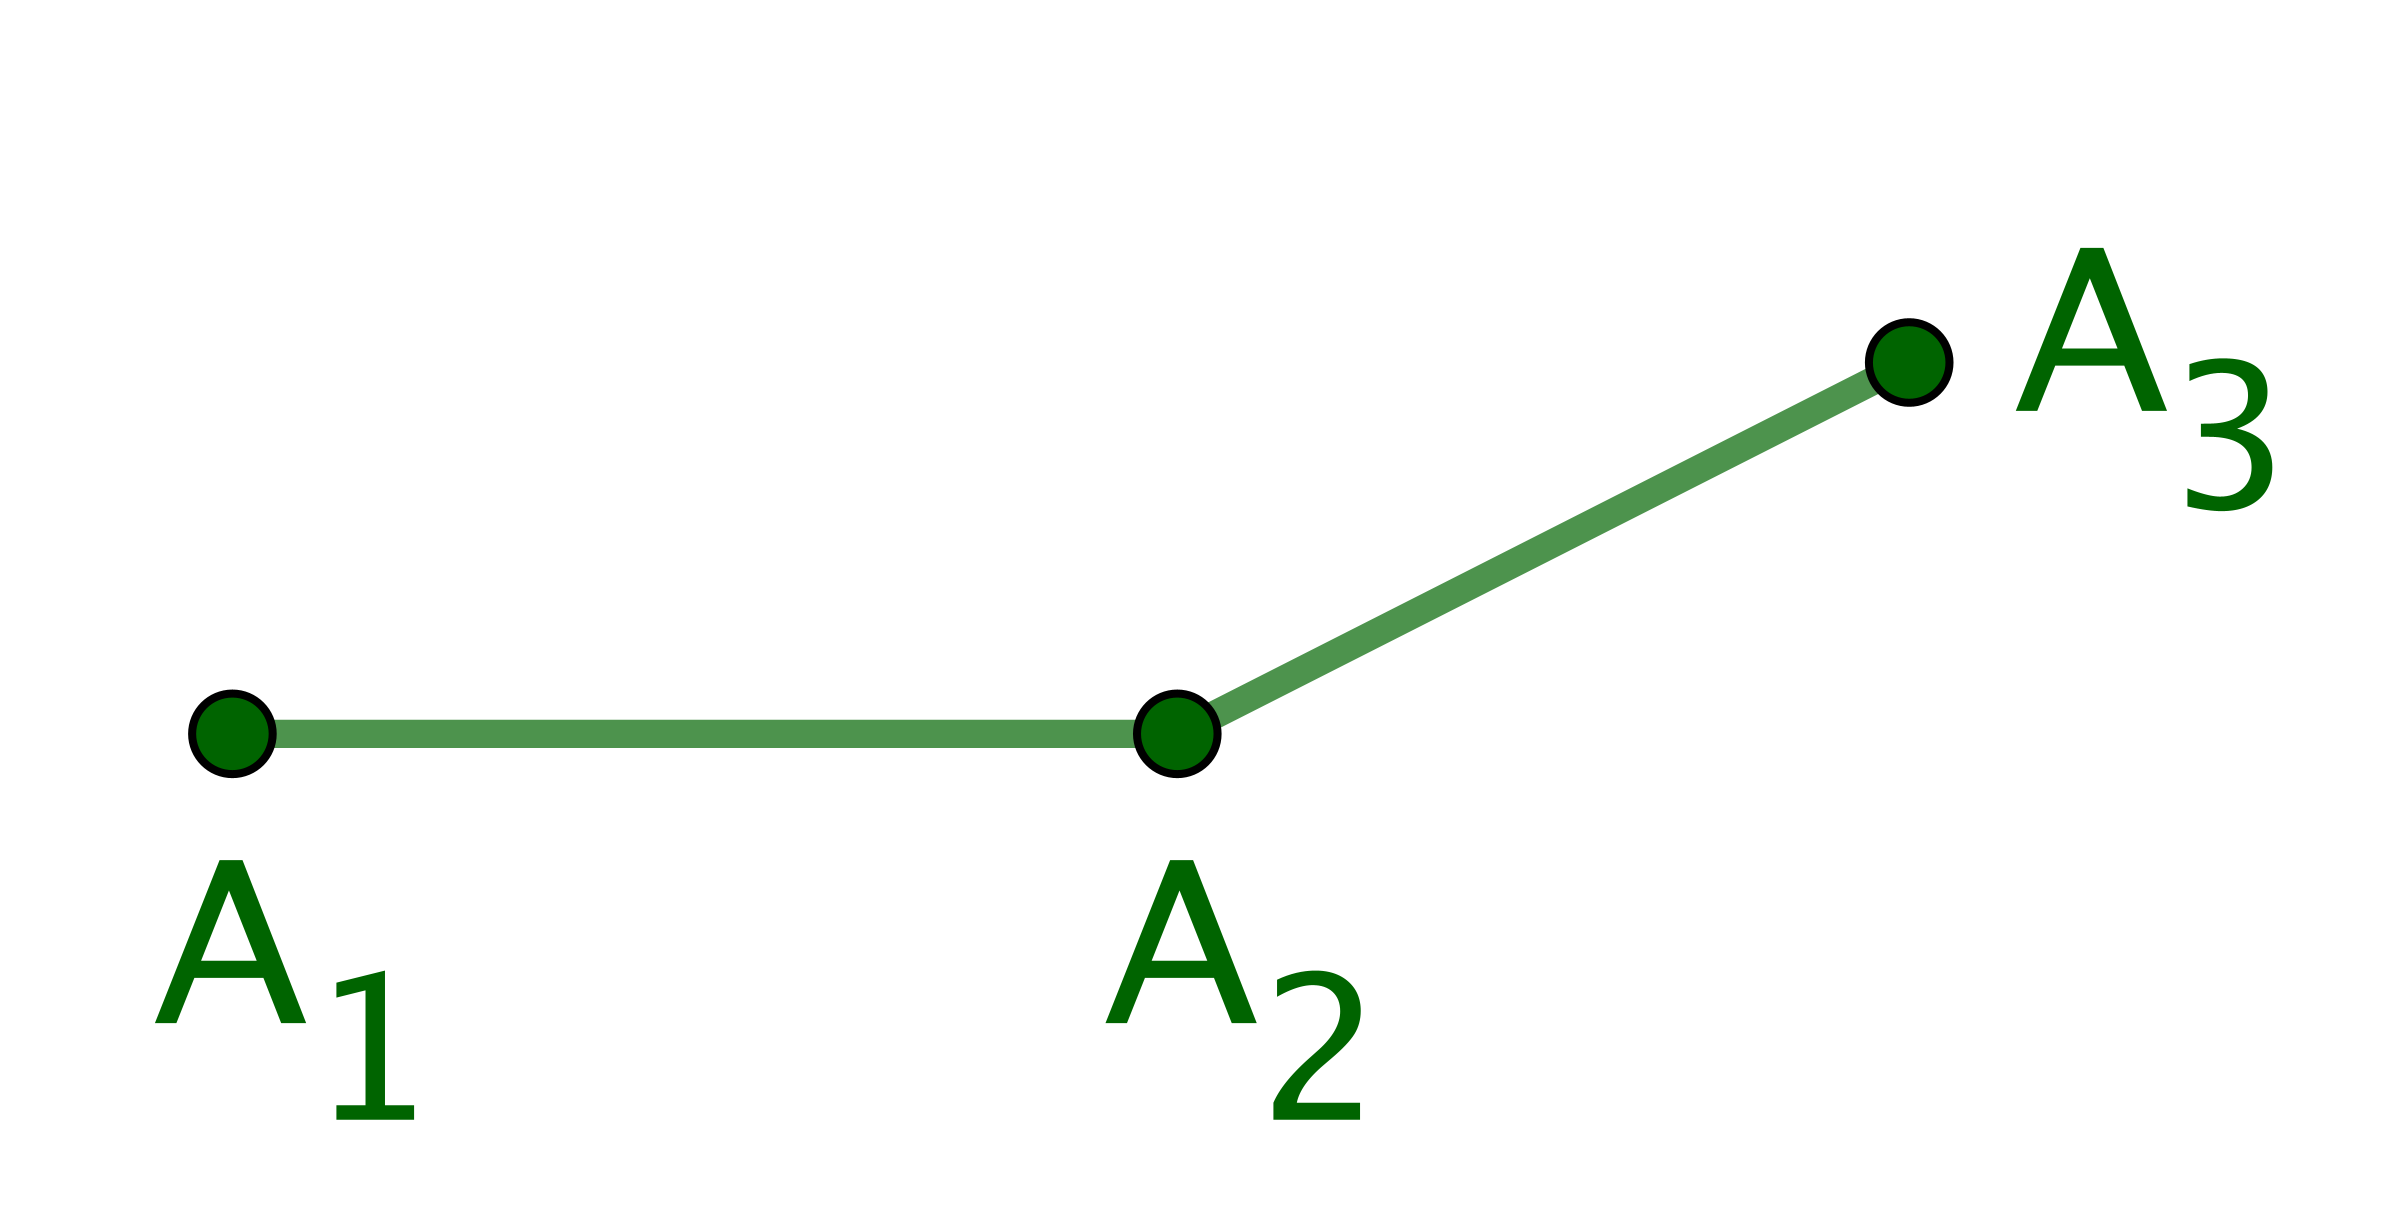
\includegraphics[scale=.45]{content/polygon/at-least-one/conv-det-sign-1.png}
    	    
    	\smallskip
        Cas positif.
        
        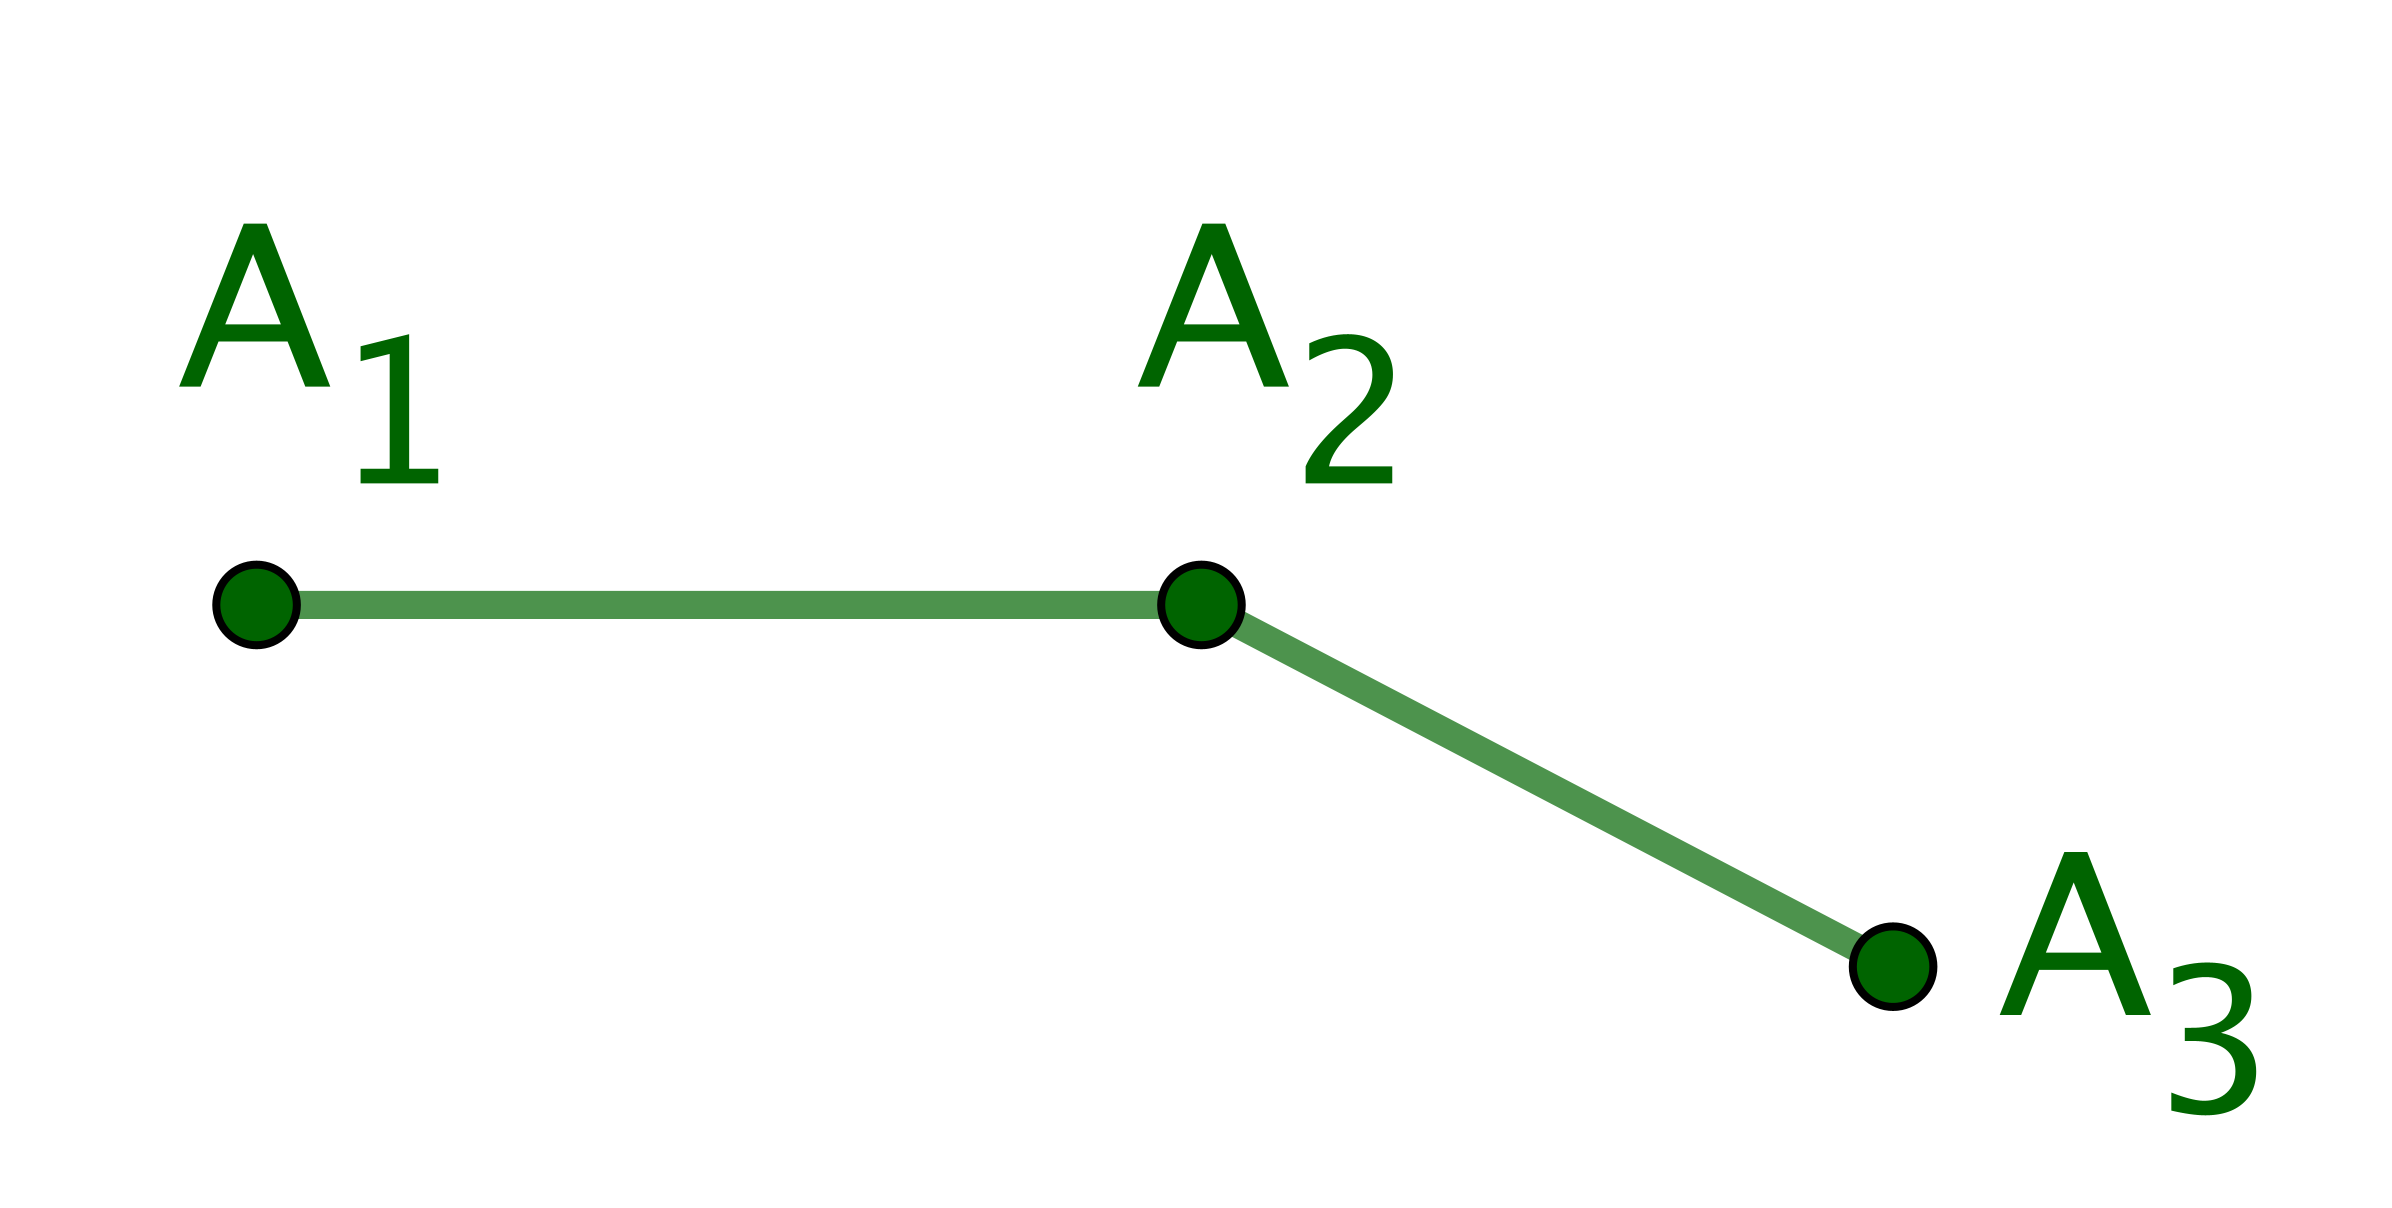
\includegraphics[scale=.45]{content/polygon/at-least-one/conv-det-sign-2.png}
    	    
    	\smallskip
        Cas négatif.
    \end{multicols}

    
    \noindent
    Considérons le cas positif, c'est-à-dire supposons que 
    $\det \big( \vect{A^{\,\prime}_1 A^{\,\prime}_2}, \vect{A^{\,\prime}_1 A^{\,\prime}_3} \big) > 0$.
	%
	\begin{itemize}
    	\item $\vect{A^{\,\prime}_1 A^{\,\prime}_3} = \vect{A^{\,\prime}_1 A^{\,\prime}_2} + \vect{A^{\,\prime}_2 A^{\,\prime}_3}$
    	donne
		$\det \big( \vect{A^{\,\prime}_2 A^{\,\prime}_3}, \vect{A^{\,\prime}_2 A^{\,\prime}_1} \big) > 0$.


		\item Comme $A_2$, $A_3$ et $A_4$ ne sont pas alignés, et de plus $A_1$ et $A_4$ du même côté, au sens large, de la droite $(A_2 A_3)$, nous obtenons
		$\det \big( \vect{A^{\,\prime}_2 A^{\,\prime}_3}, \vect{A^{\,\prime}_2 A^{\,\prime}_4} \big) > 0$.


		\item En continuant de proche en proche, nous arrivons à
		$\det \big( \vect{A^{\,\prime}_i A^{\,\prime}_{i+1}}, \vect{A^{\,\prime}_i A^{\,\prime}_{i+2}} \big) > 0$
		pour $i \in \ZintervalC{1}{n}$ quelconque.


		\item Le point précédent et la convexité donnent
		$\det \big( \vect{A^{\,\prime}_i A^{\,\prime}_{i+1}}, \vect{A^{\,\prime}_i A^{\,\prime}_k} \big) \geq 0$
		pour $(i, k) \in \ZintervalC{1}{n}^2$ tel que $k \notin \setgene{i ; i+1}$.


		\item
		Montrons maintenant que
		$\det \big( \vect{A^{\,\prime}_1 A^{\,\prime}_2}, \vect{A^{\,\prime}_1 A^{\,\prime}_k} \big) > 0$
		pour $k \in \ZintervalC{3}{n}$.
		%
		Nous savons déjà l'inégalité vraie pour $k = 3$, donc passons à $k = 4$.
		Pour avoir 
		$\det \big( \vect{A^{\,\prime}_1 A^{\,\prime}_2}, \vect{A^{\,\prime}_1 A^{\,\prime}_k} \big) > 0$, 
		le point précédent donne qu'il faut vérifier que 
		$\det \big( \vect{A^{\,\prime}_1 A^{\,\prime}_2}, \vect{A^{\,\prime}_1 A^{\,\prime}_k} \big) = 0$
		est impossible.
		Supposons donc l'égalité vraie, ce qui implique d'avoir $n \geq 5$, et donne les configurations suivantes où les hachures et la droite en trait plein sont des zones interdites pour $A_4$.

        \begin{multicols}{2}
            \small\itshape\centering
           	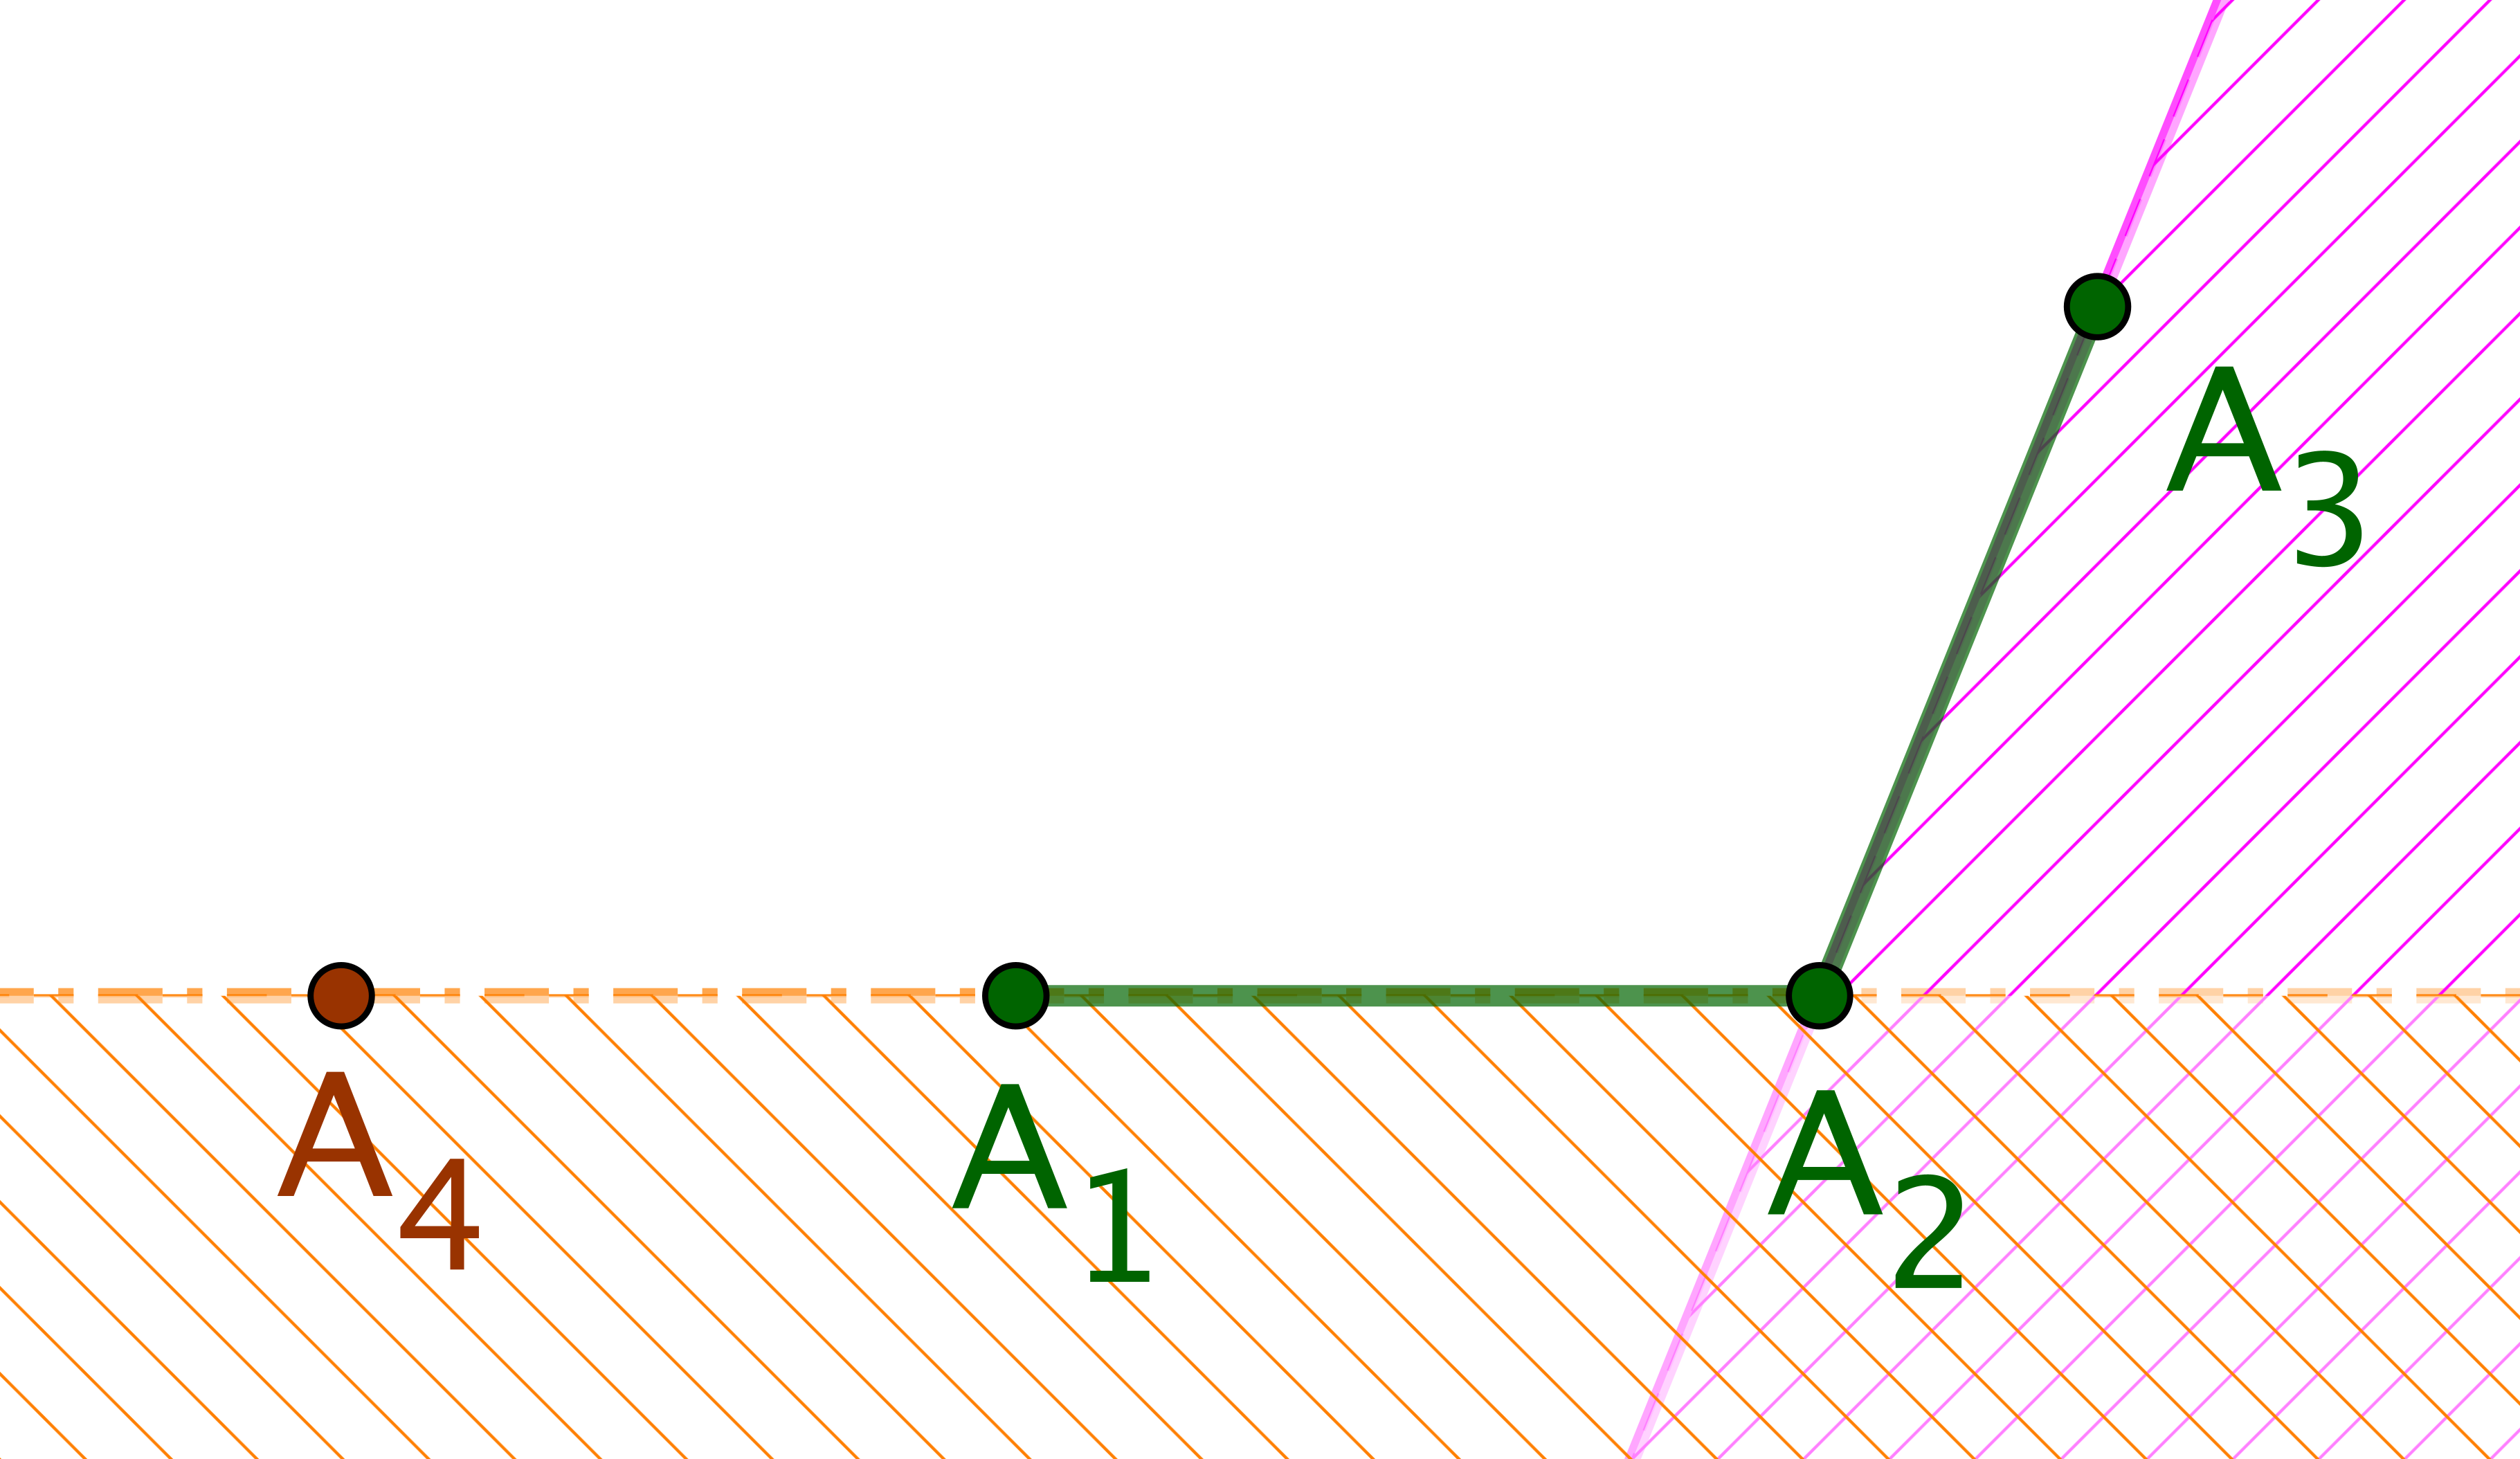
\includegraphics[scale=.4]{content/polygon/at-least-one/conv-det-A4-1.png}
        	    
        	\smallskip
            Cas 1.
            
            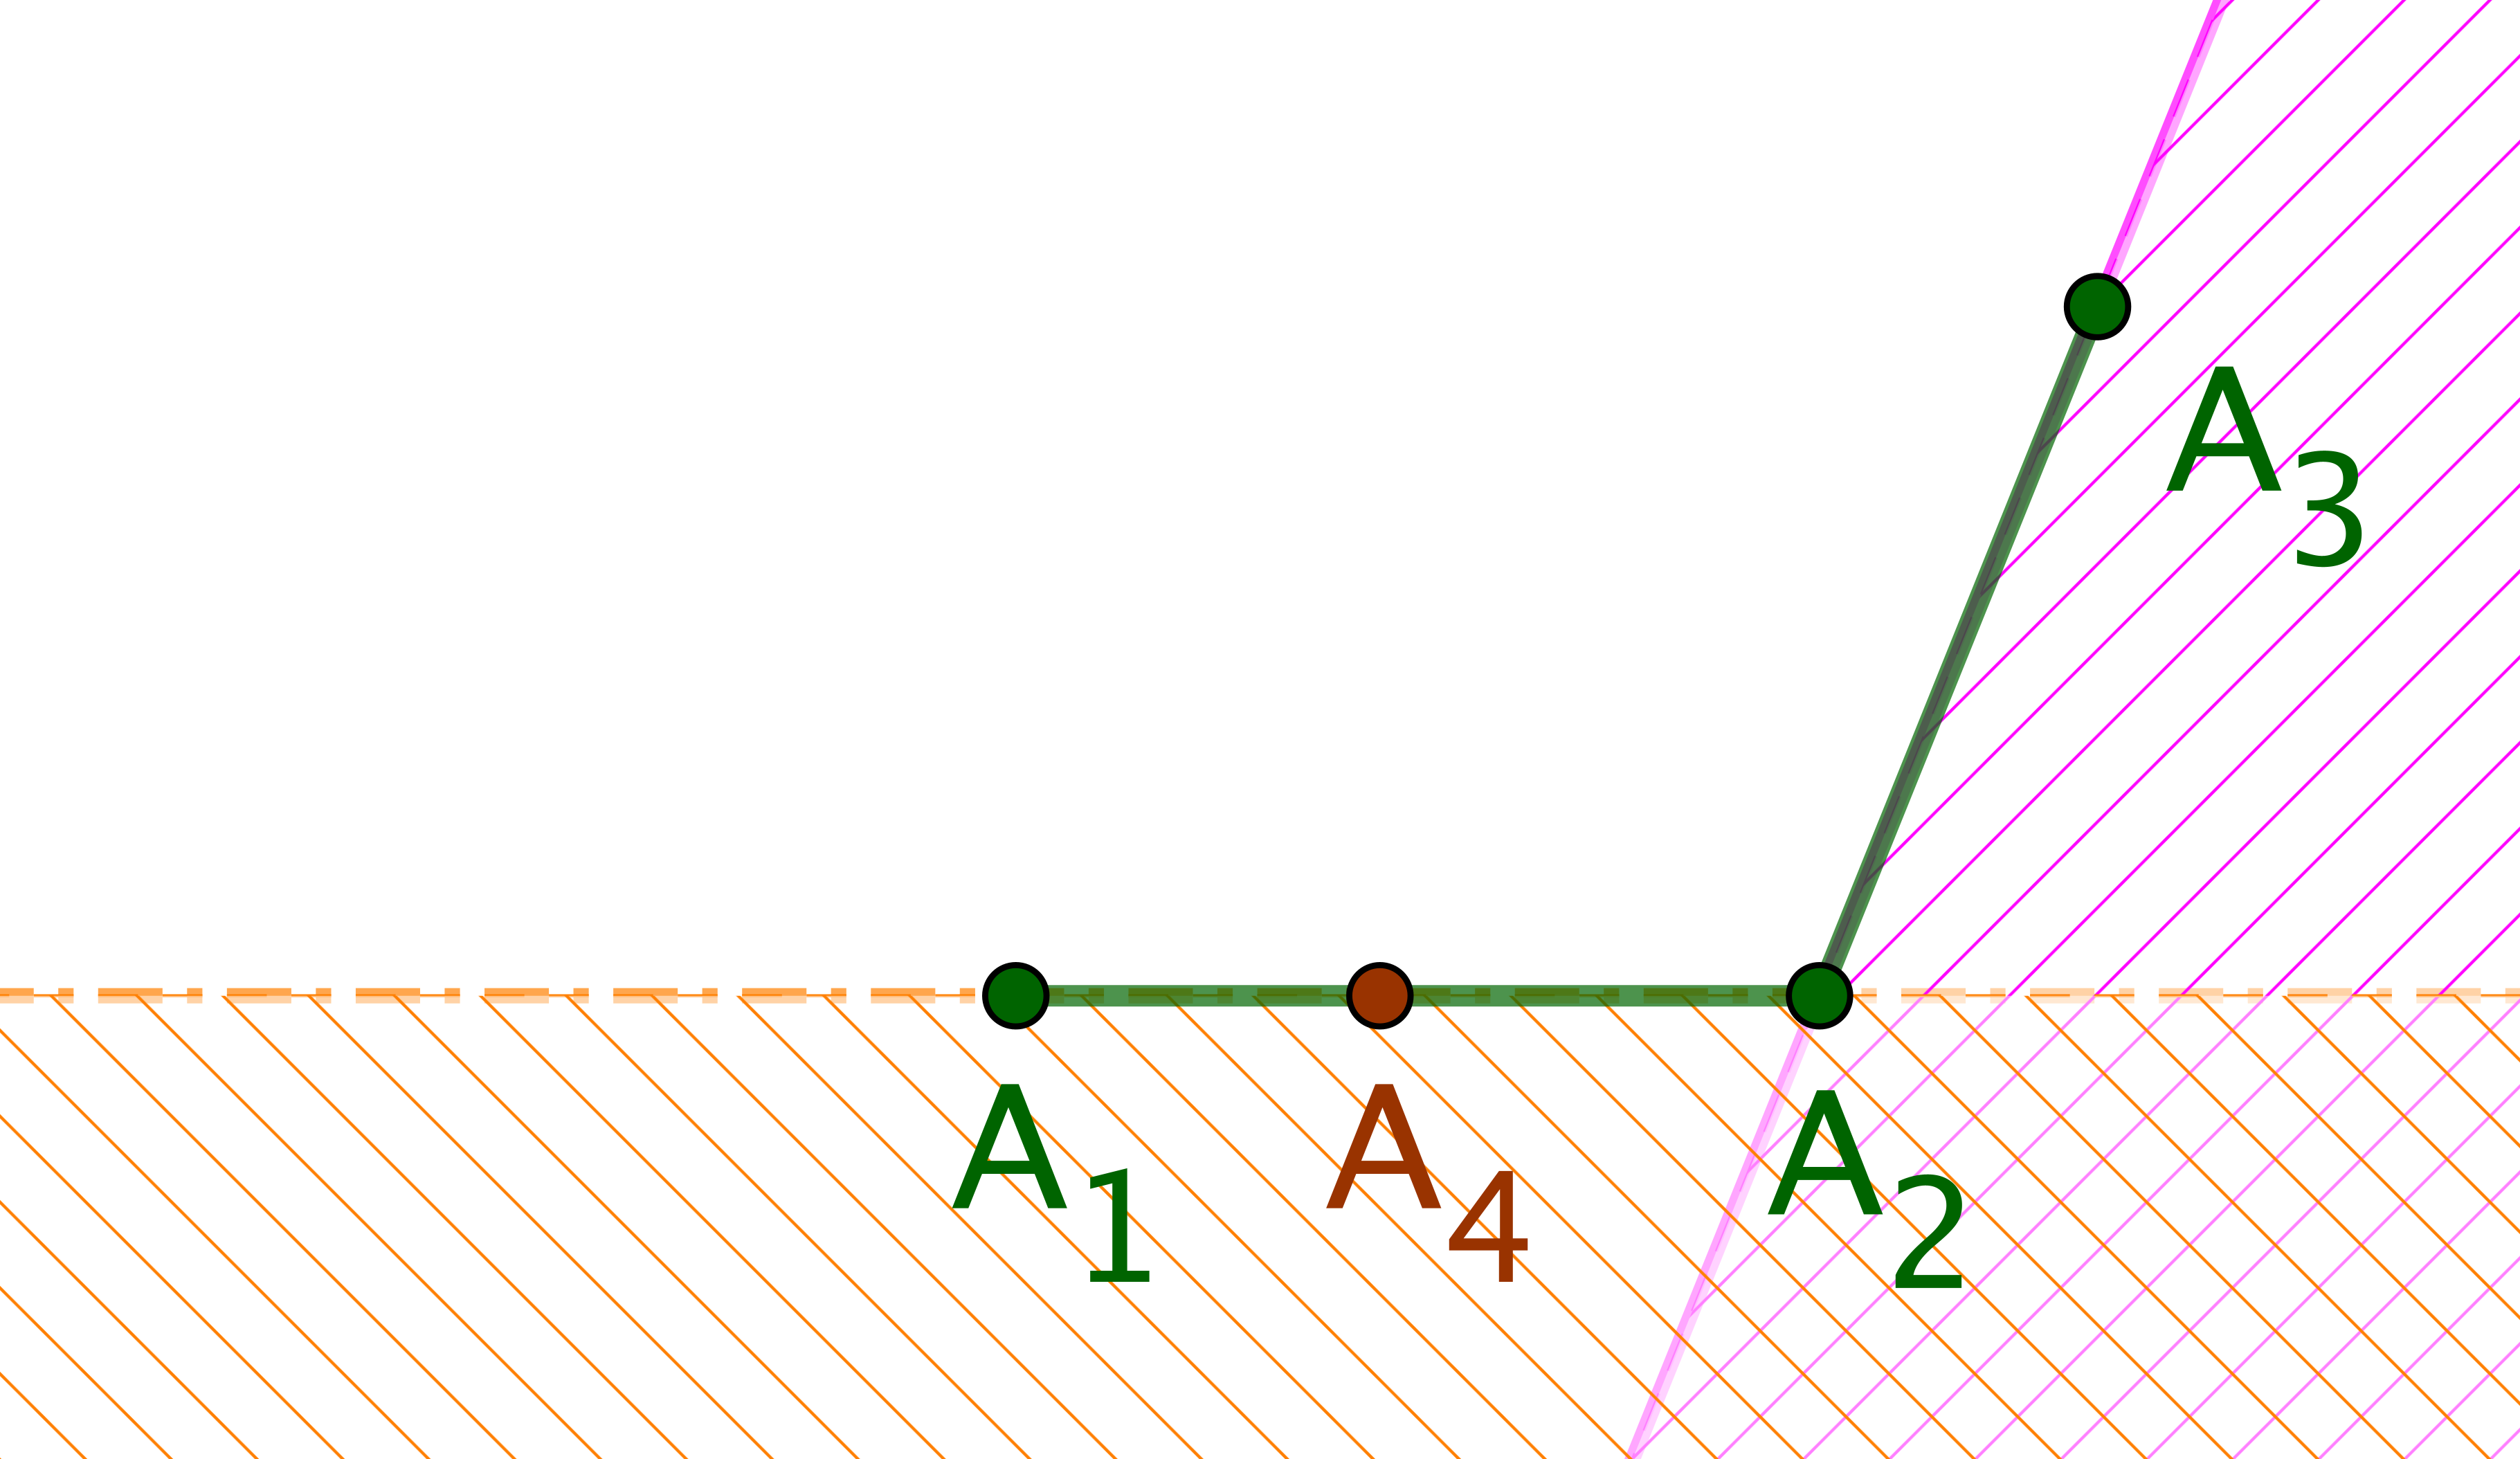
\includegraphics[scale=.4]{content/polygon/at-least-one/conv-det-A4-2.png}
        	    
        	\smallskip
            Cas 2.
        \end{multicols}
    
		\noindent
		Le cas 2 est impossible par raison de convexité, car $A_1$ et $A_2$ sont de part et d'autre de la droite $(A_3 A_4)$. Voyons donc ce qu'implique le 1\ier\ cas pour $A_5$.
		
        \begin{multicols}{2}
            \small\itshape\centering
           	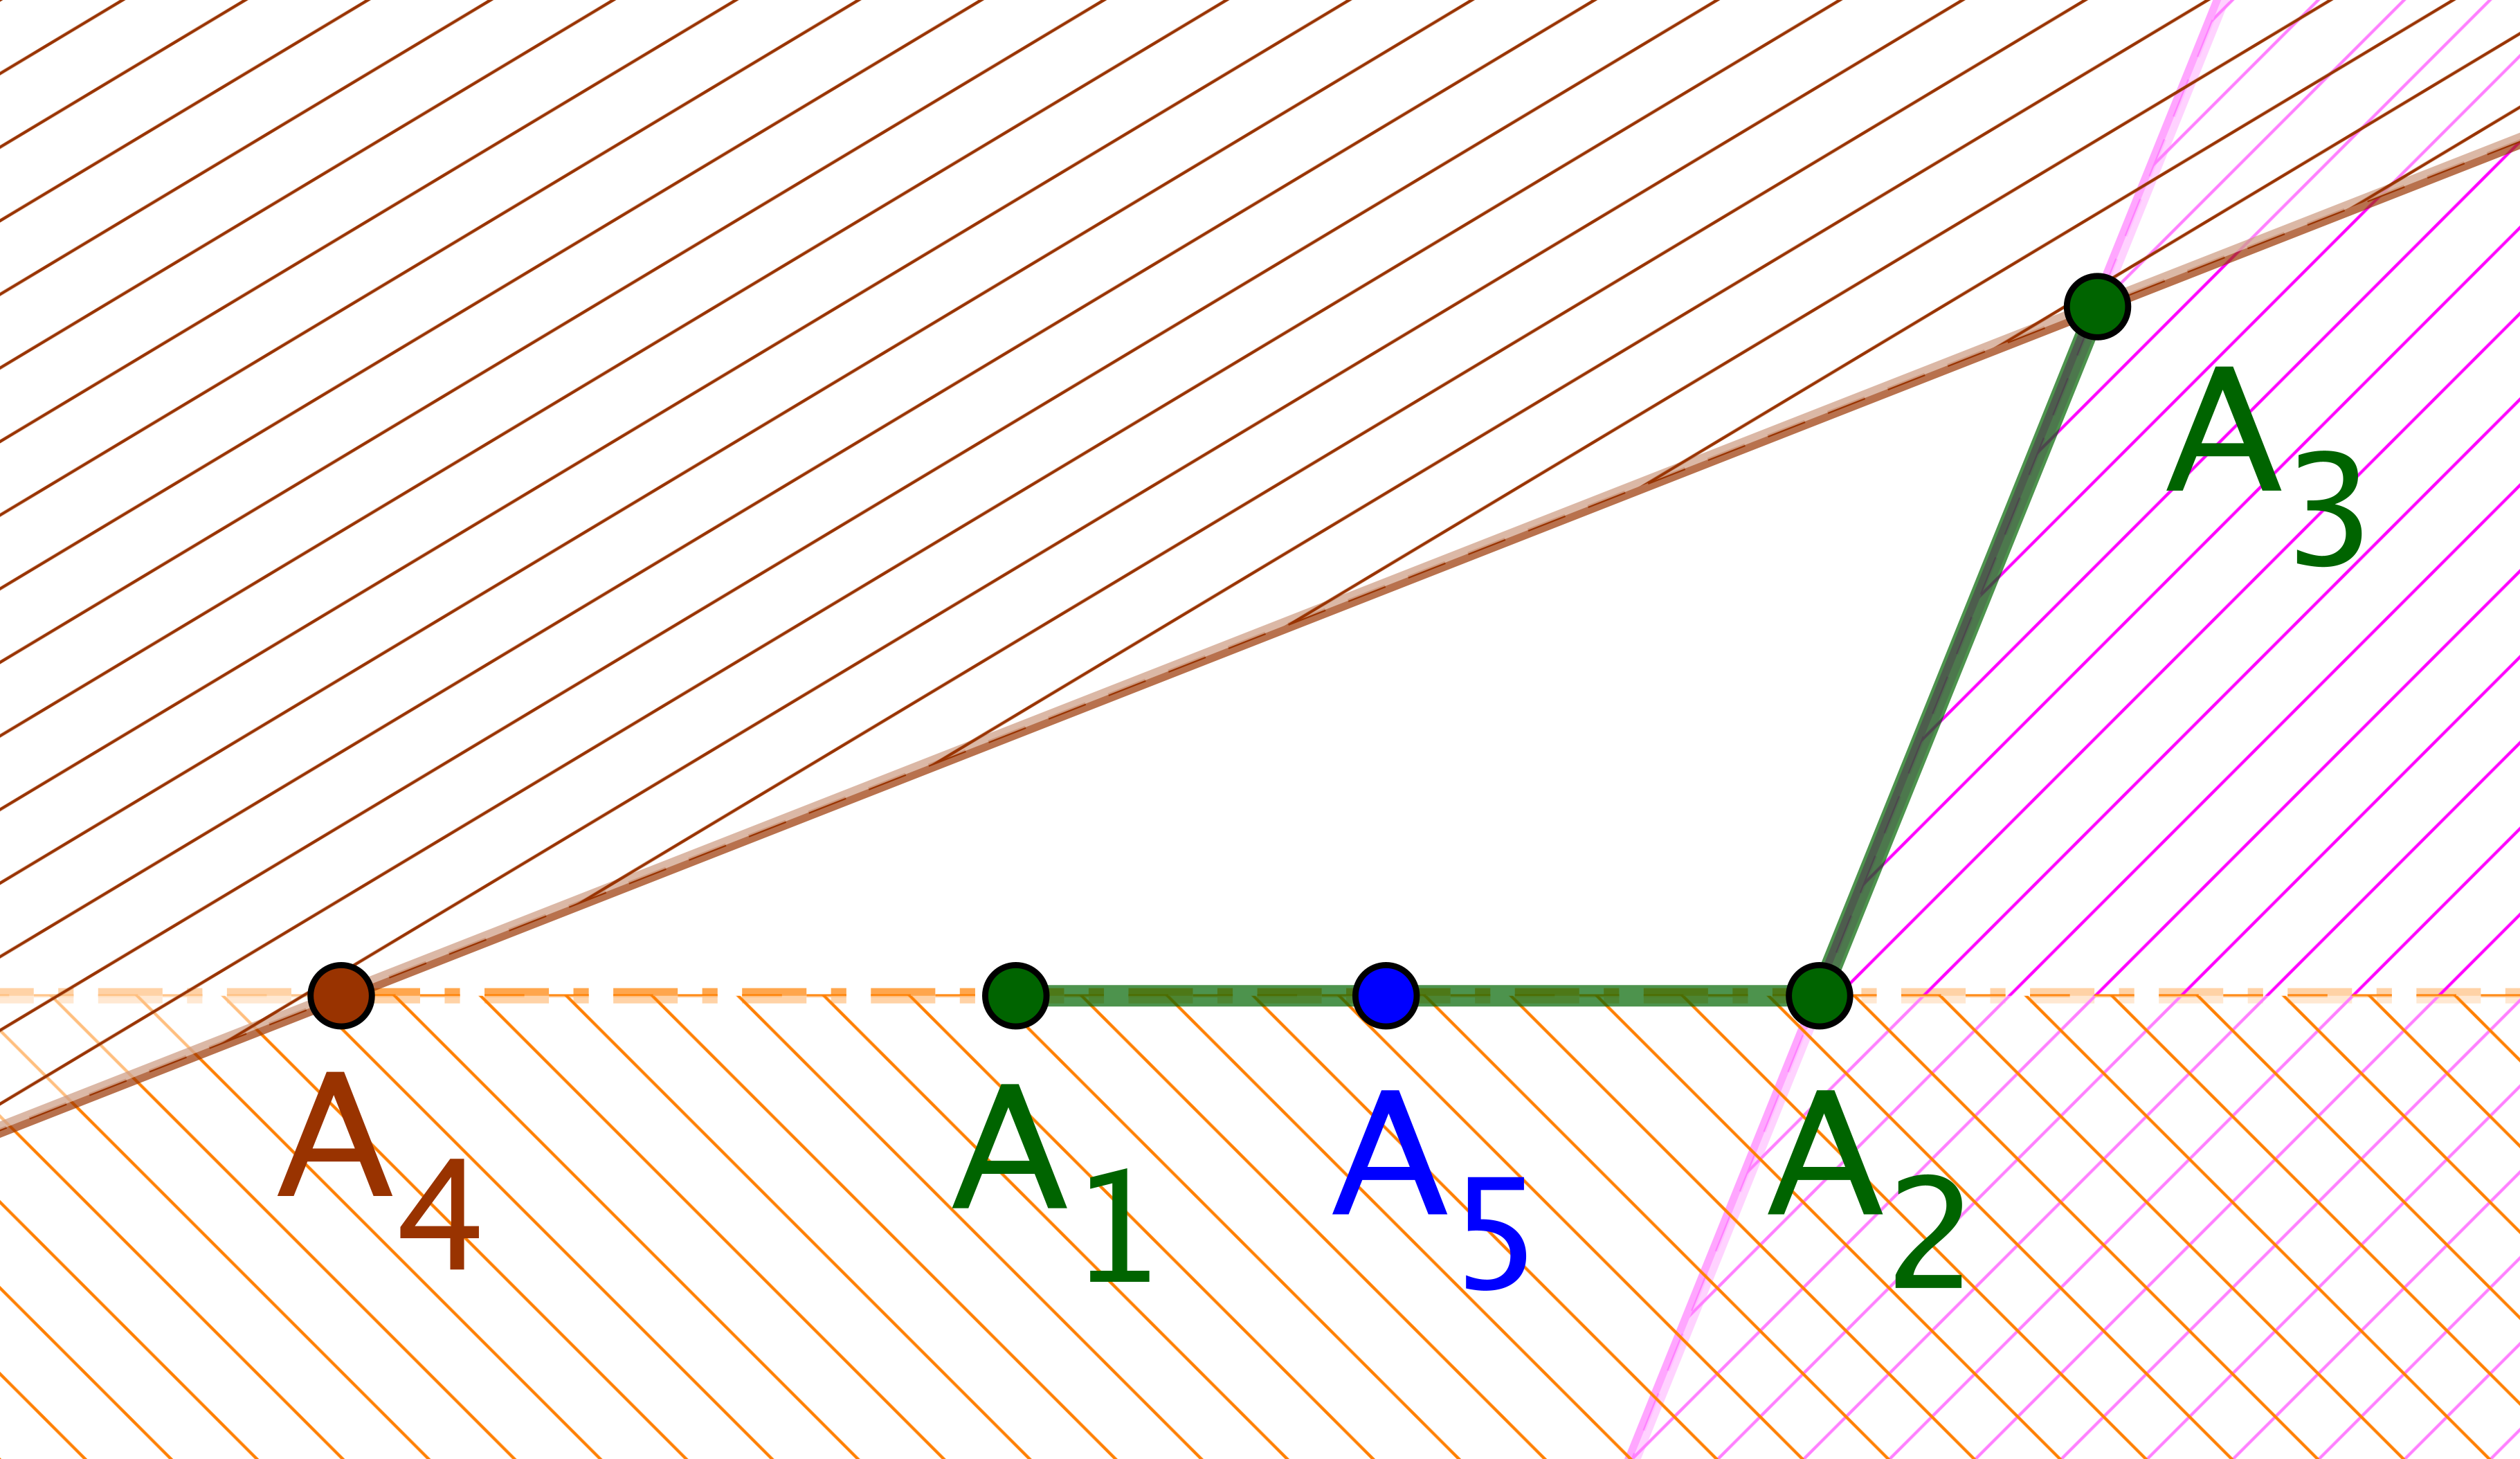
\includegraphics[scale=.4]{content/polygon/at-least-one/conv-det-A5-1.png}
        	    
        	\smallskip
            Cas 1-1.
            
            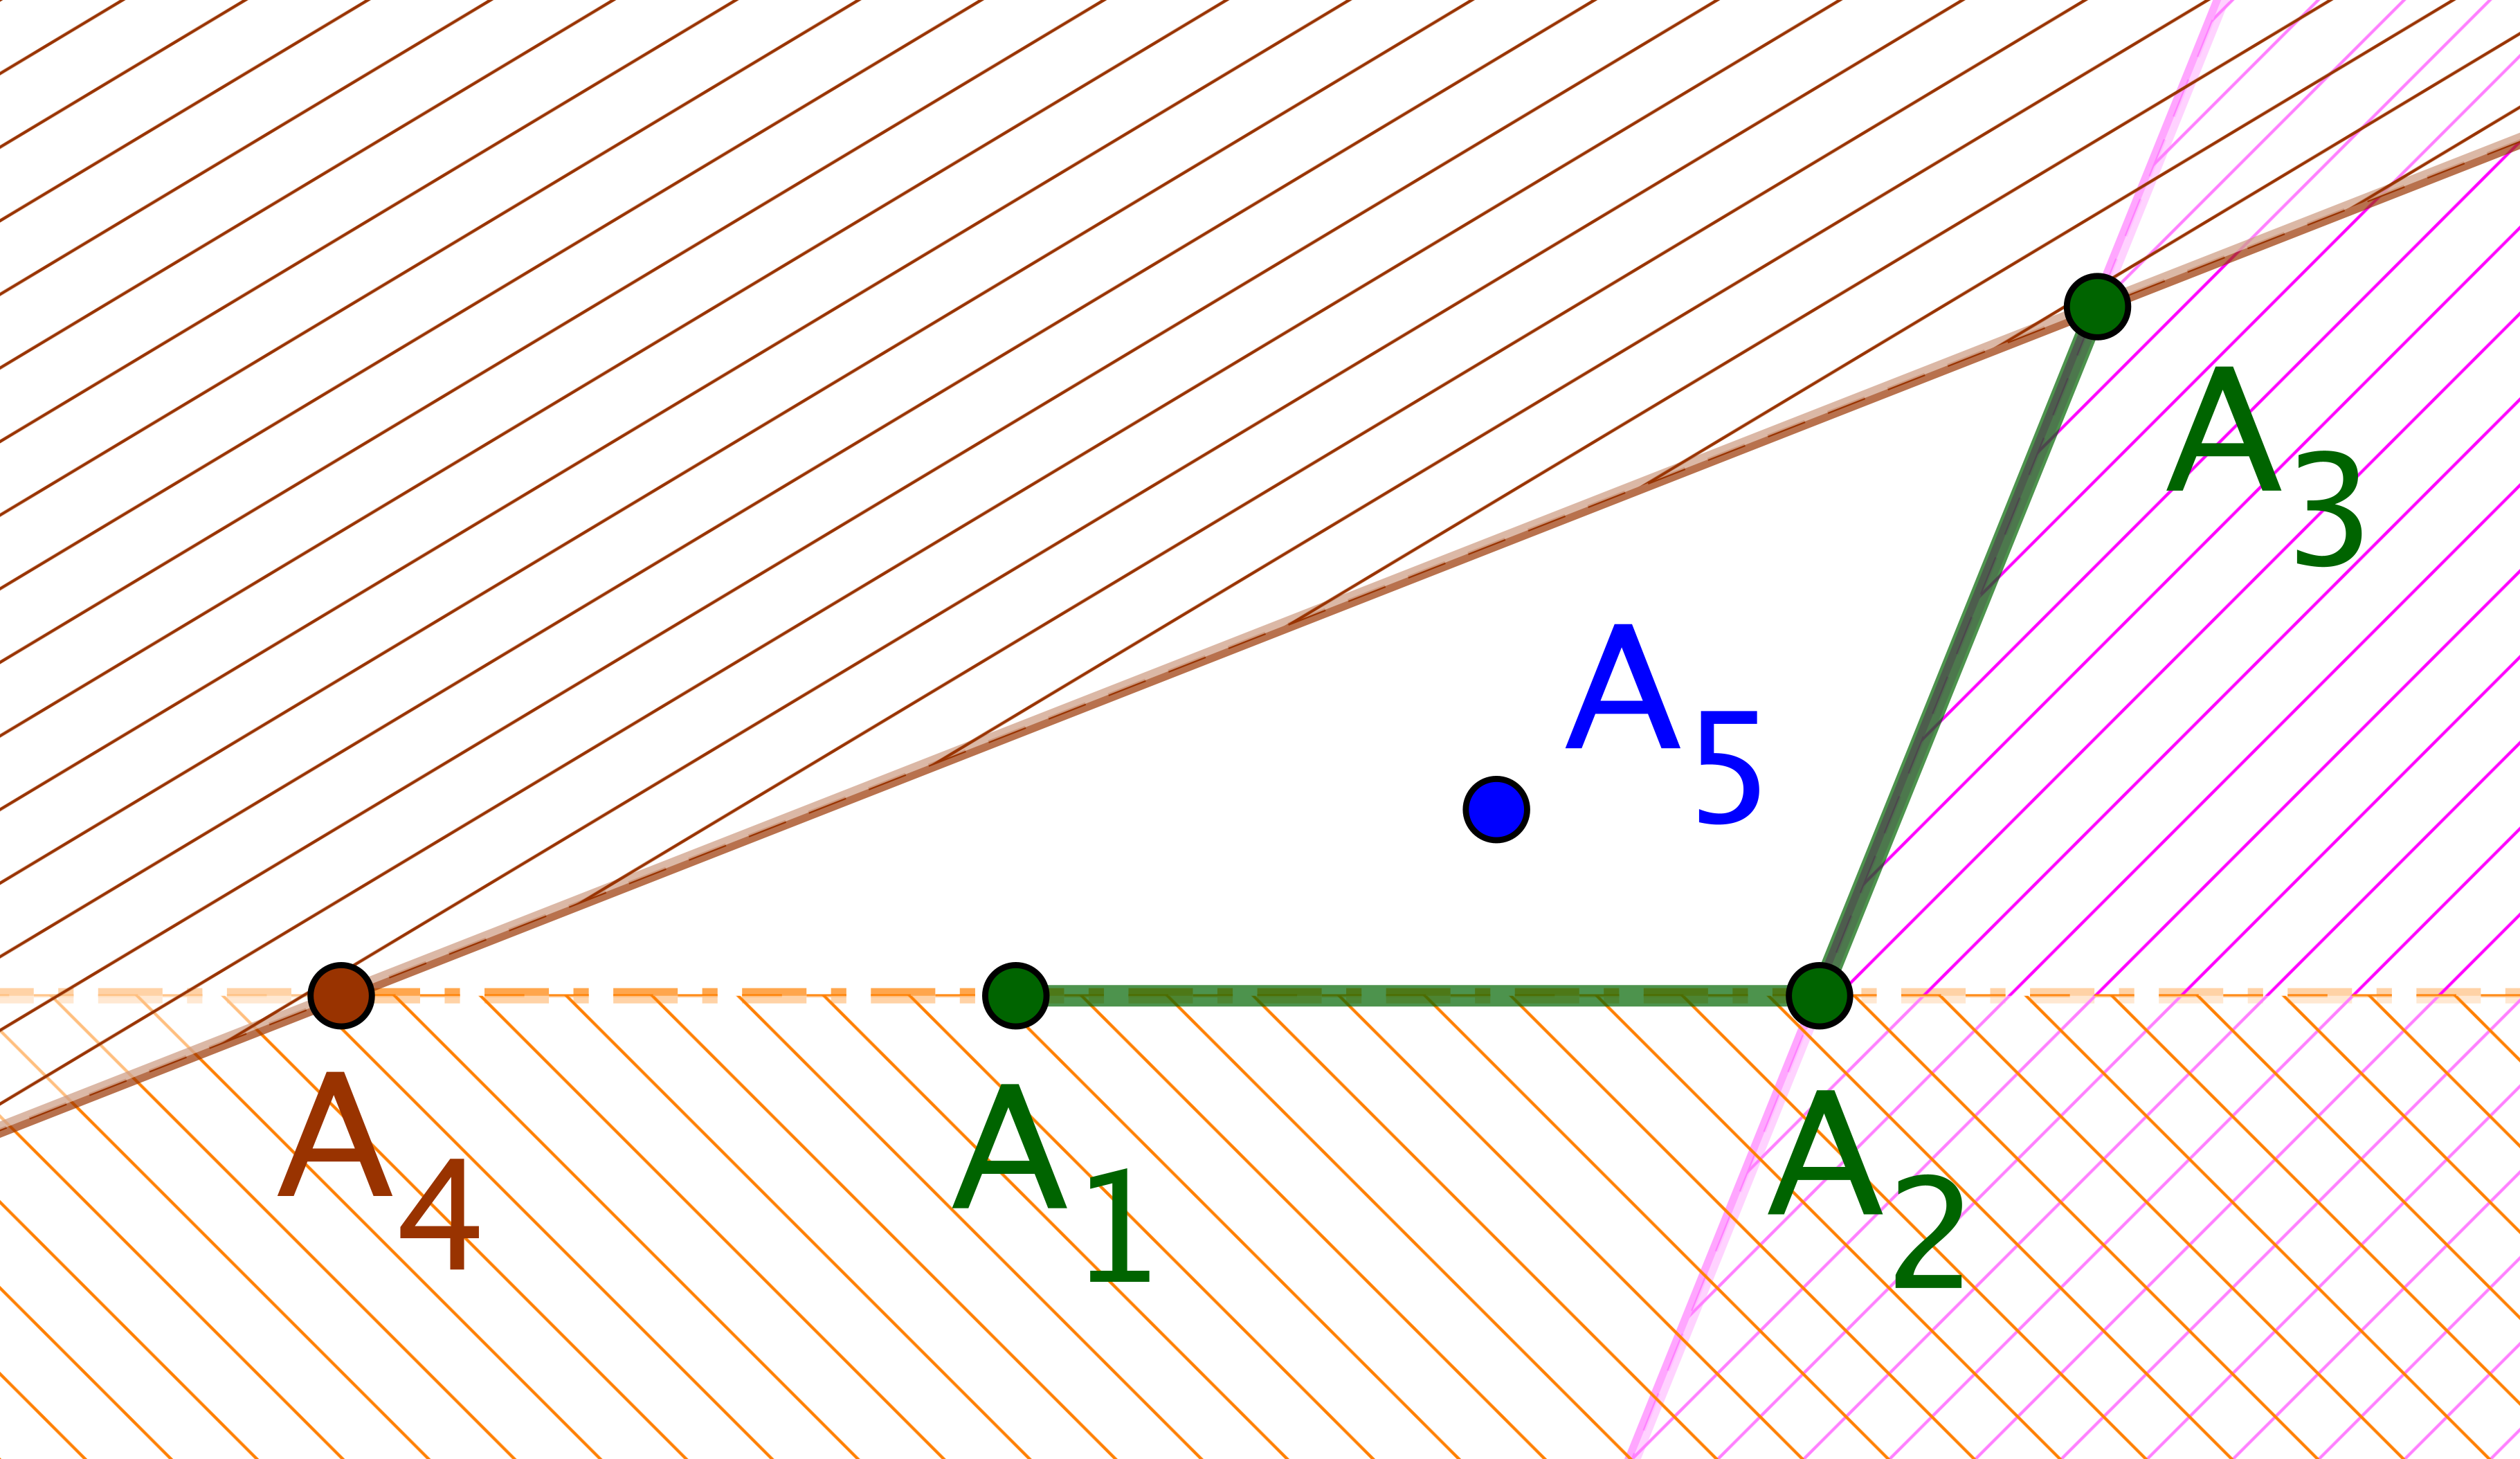
\includegraphics[scale=.4]{content/polygon/at-least-one/conv-det-A5-2.png}
        	    
        	\smallskip
            Cas 1-2.
        \end{multicols}
    
		\noindent
		Le cas 1-2 est impossible par raison de convexité à cause de $(A_4 A_5)$.
		Notons que dans le cas 1-1, il est possible d'avoir $A_5 \in ]A_4 A_1[$.
		Comme $A_5 \in (A_1 A_2)$, nous devons avoir $n \geq 6$.
		Dès lors, nous avons de nouveau $A_6 \in (A_1 A_2)$, mais ceci donne la contradiction $A_6 \in (A_4 A_5)$.
		Continuons ensuite de proche en proche, nous obtenons bien
		$\det \big( \vect{A^{\,\prime}_1 A^{\,\prime}_2}, \vect{A^{\,\prime}_1 A^{\,\prime}_k} \big) > 0$
		pour $k \in \ZintervalC{3}{n}$.


		\item En généralisant le raisonnement précédent,%
		\footnote{
		    Se souvenir de la définition de la suite $(A^{\,\prime}_i)$.
		}
		nous avons
		$\det \big( \vect{A^{\,\prime}_i A^{\,\prime}_{i+1}}, \vect{A^{\,\prime}_i A^{\,\prime}_k} \big) > 0$
		pour tout couple $(i, k) \in \ZintervalC{1}{n}^2$ vérifiant $k \notin \setgene{i ; i+1}$.
	\end{itemize}


    \noindent
    Le cas négatif se traite de façon similaire.
\end{proof}


% ----------------------- %


\newpage


Nous allons établir une réciproque élargie du résultat précédent. Ce nouveau fait va nous rendre un grand service par la suite.%
\footnote{
    Pourquoi s'attarder sur des inégalités larges? Parce que nous allons travailler dans un ensemble compact, et donc fermé, de \ncycles.
    Pour garder des \ngones, nous devrions utiliser des non-égalités, mais ceci nous ferait sortir du cadre fermé qui nous intéresse.
    Nous n'avons pas le choix!
}


\begin{fact} \label{conv-from-non-neg-det}
    Soit $\setproba{L} = A_1 A_2 \cdots A_n$ un \ncycle\ vérifiant l'une des alternatives suivantes.
    %
	\begin{itemize}
		\item $\forall (i, k) \in \ZintervalC{1}{n}^2$,
		$\det \big( \vect{A^{\,\prime}_i A^{\,\prime}_{i+1}}, \vect{A^{\,\prime}_i A^{\,\prime}_k} \big) \geq 0$.

		\item $\forall (i, k) \in \ZintervalC{1}{n}^2$,
		$\det \big( \vect{A^{\,\prime}_i A^{\,\prime}_{i+1}}, \vect{A^{\,\prime}_i A^{\,\prime}_k} \big) \leq 0$.
    \end{itemize}
    
    Ceci implique la validité de l'une des assertions ci-dessous.
    %
	\begin{enumerate}[label=\roman*.]
		\item $\setproba{L}$ est totalement dégénéré.

		\item Il existe un \kgone\ convexe $\setproba{C}$ tel que
		$k \leq n$, 
		$\cyclelen{\setproba{C}} \leq \cyclelen{\setproba{L}}$
		et
		$\sarea{\setproba{C}} = \sarea{\setproba{L}}$,
		ceci se faisant en retirant, si nécessaire, des sommets de $\setproba{L}$, sans modifier l'ordre de parcours pour les sommets gardés.
    \end{enumerate}
\end{fact}


\begin{proof}
    Par symétrie des alternatives, nous pouvons nous concentrer sur le cas positif, c'est-à-dire supposer que
    $\forall (i, k) \in \ZintervalC{1}{n}^2$,
	$\det \big( \vect{A^{\,\prime}_i A^{\,\prime}_{i+1}}, \vect{A^{\,\prime}_i A^{\,\prime}_k} \big) \geq 0$.
	%
	Seul le cas $\setproba{L}$ non totalement dégénéré demande notre attention.
	Nous allons raisonner algorithmiquement en utilisant
	une variable $i$ initialisée à $1$, 
	et une liste $\onelist{C}$, initialement vide, pour stocker les sommets \og utiles \fg\ à la fabrication du \kgone\ convexe final.
	Notons que la non totale dégénérescence donne que 
    $\forall i \in \ZintervalC{1}{n}$,
    $\exists k \in \ZintervalC{1}{n}$
    tel que
	$\det \big( \vect{A^{\,\prime}_i A^{\,\prime}_{i+1}}, \vect{A^{\,\prime}_i A^{\,\prime}_k} \big) > 0$.
	%
	\begin{enumerate}[label=\fbox{\small\bfseries\textsf{A\kern.25pt\arabic*}}]
    	\item \label{start-algo-extract-kgone}
	    Si 
		$\det \big( \vect{A^{\,\prime}_i A^{\,\prime}_{i+1}}, \vect{A^{\,\prime}_i A^{\,\prime}_{i+1}} \big) > 0$,
		nous ajoutons $i$ à la fin de la liste $\onelist{C}$,
		puis nous passons directement à l'action \ref{next-algo-extract-kgone}\,.


    	\item Sinon, il existe 
	    $m \in \ZZ_{>i+1}$ minimal tel que
		$\det \big( \vect{A^{\,\prime}_i A^{\,\prime}_{i+1}}, \vect{A^{\,\prime}_i A^{\,\prime}_m} \big) > 0$.%
		\footnote{
		    Voir la remarque juste avant le présent algorithme.
		}
        %
        \begin{center}
        	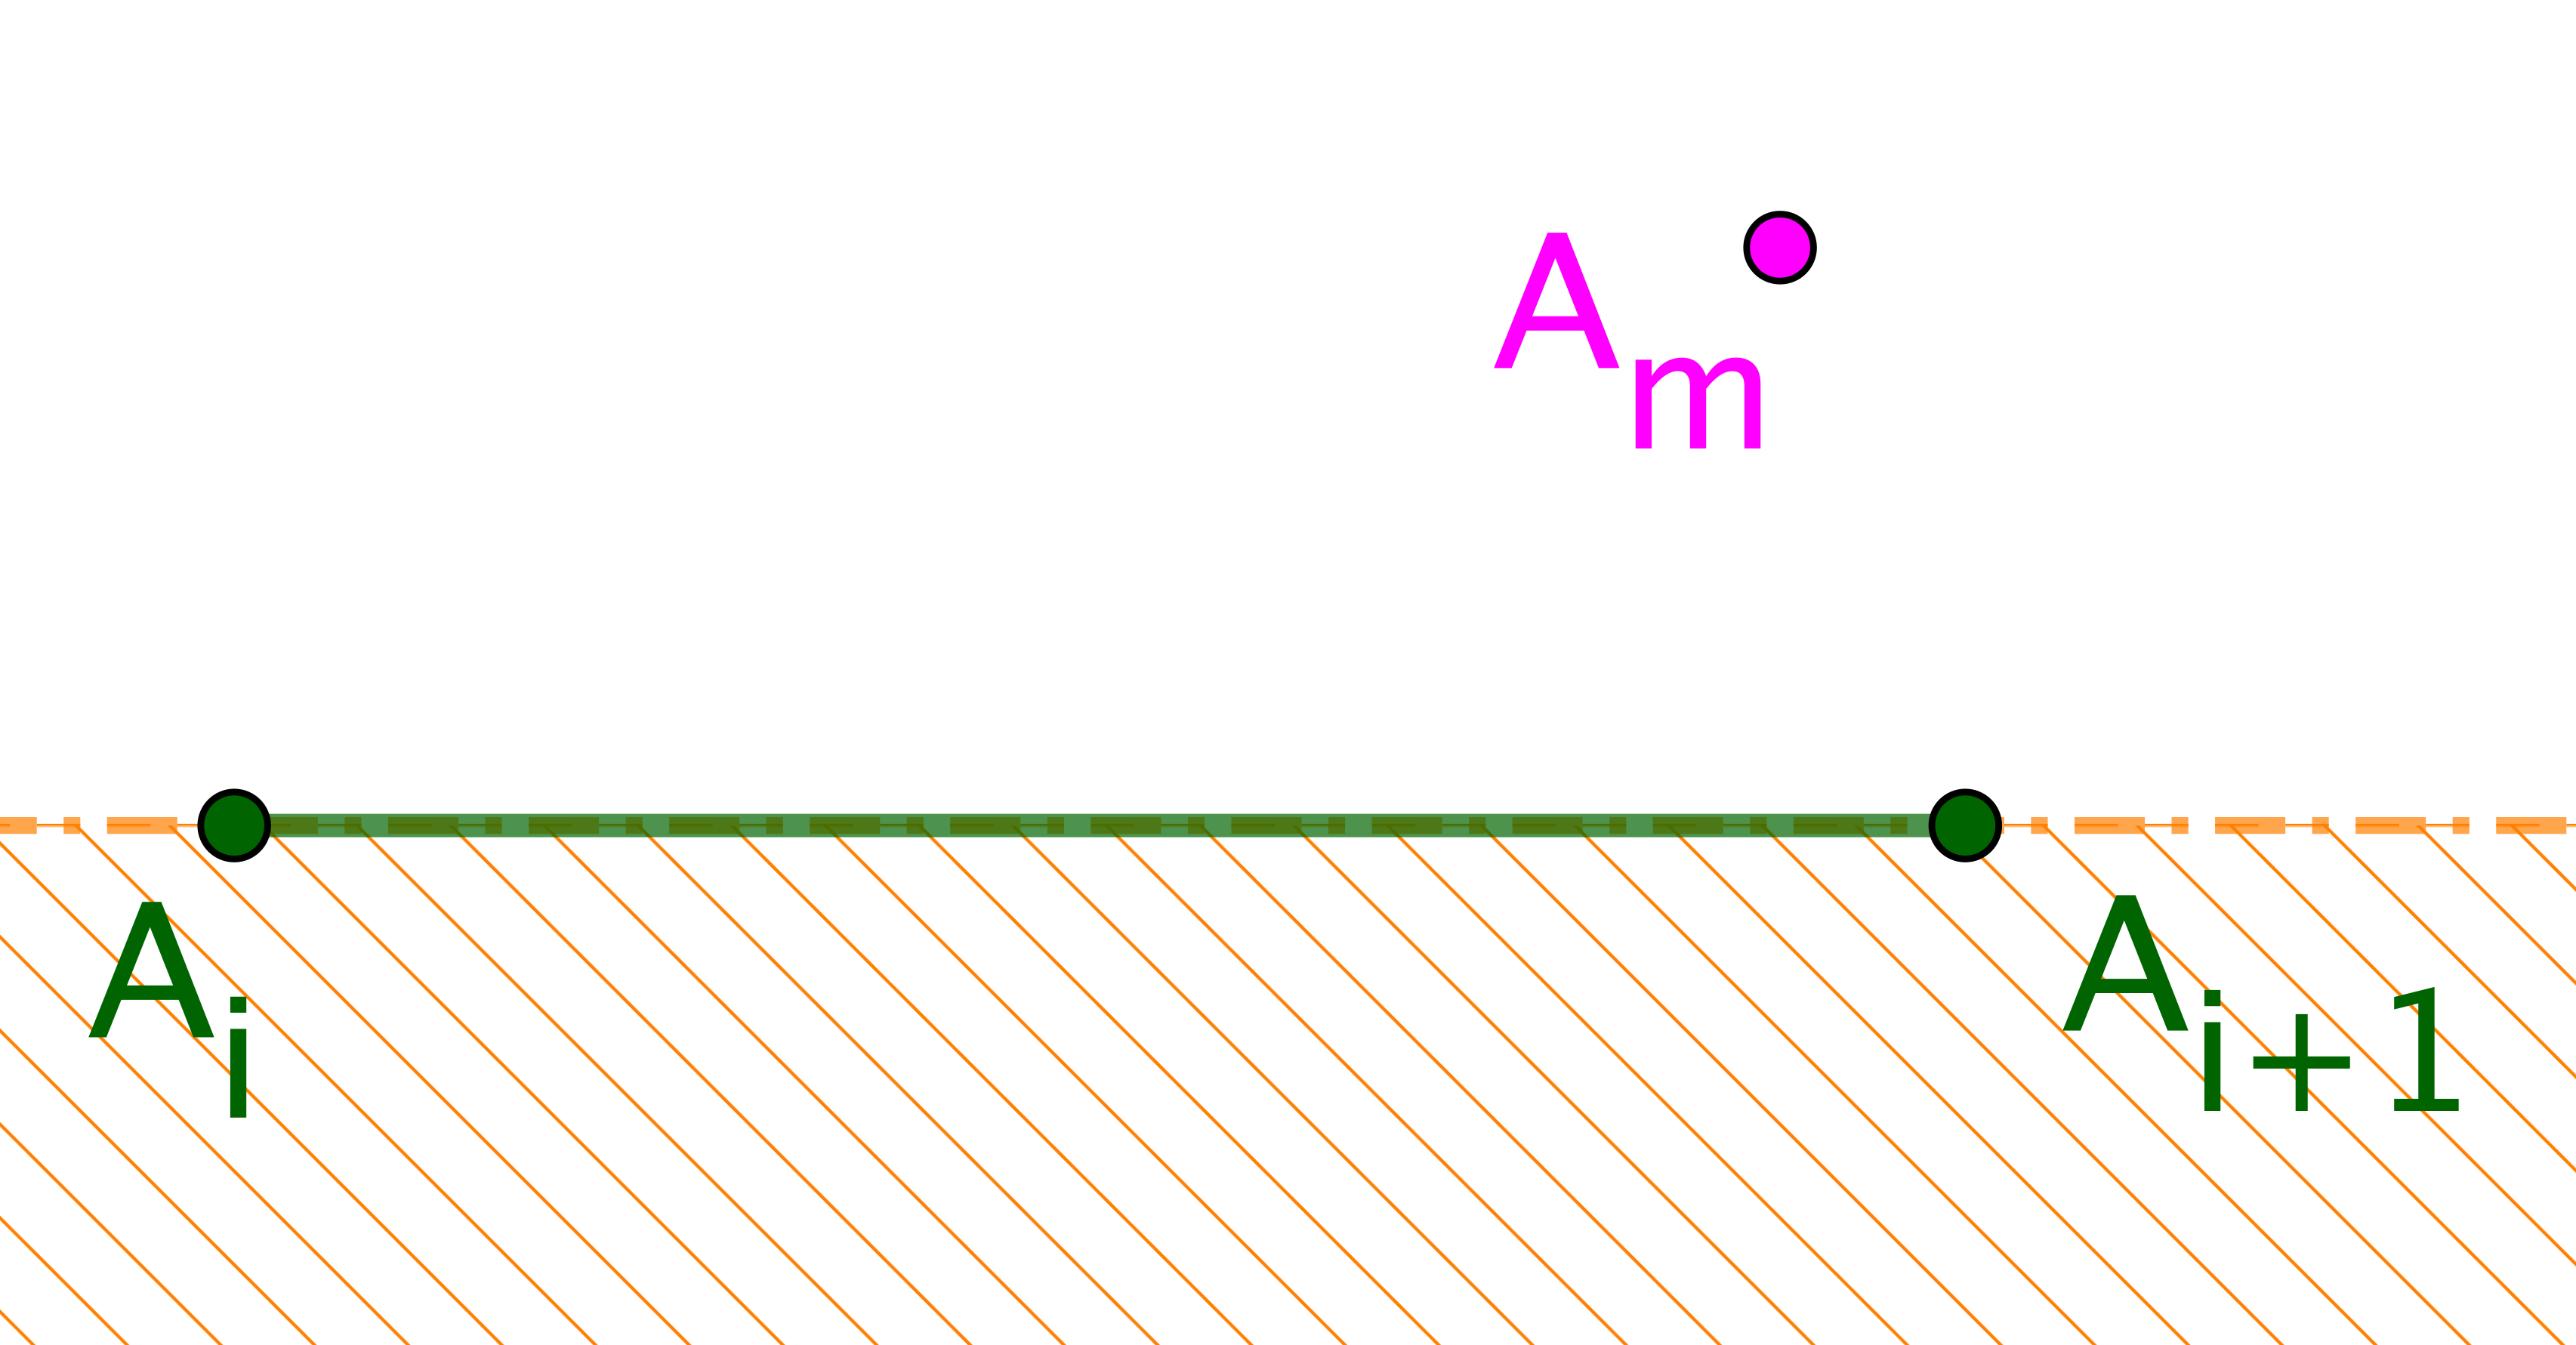
\includegraphics[scale=.4]{content/polygon/at-least-one/next-extract-kgone.png}
        \end{center}
        
        \noindent
        Comme 
        $\det \big( \vect{A^{\,\prime}_{m-1} A^{\,\prime}_m}, \vect{A^{\,\prime}_{m-1} A^{\,\prime}_{i+1}} \big) \geq 0$, 
        forcément 
        $A^{\,\prime}_{m-1} \in (A^{\,\prime}_i A^{\,\prime}_{i+1}) - (A^{\,\prime}_i A^{\,\prime}_{i+1}[$ 
        où il est possible d'avoir $A^{\,\prime}_{m-1} = A^{\,\prime}_{i+1}$.
        Nous pouvons alors faire les constations suivantes.
        %
        \begin{itemize}
            \item Les points $A^{\,\prime}_i$, $A^{\,\prime}_{m-1}$ et $A^{\,\prime}_m$ ne sont pas alignés.

            \item L'évaluation de l'aire algébrique via le point de calcul $A^{\,\prime}_{m-1}$ n'a pas besoin de tenir compte des sommets $A^{\,\prime}_j$ pour $j \in \ZintervalO{i+1}{m-1}$.

            \item Ignorer les sommets comme ci-dessus fait diminuer la valeur de la longueur.
        \end{itemize}
        
        \noindent
        Ceci justifie l'ajout de $(m-1)$ à la fin de la liste $\onelist{C}$, puis de poser $i = m-1$.

	
		\item \label{next-algo-extract-kgone}
		Ajoutons $1$ à $i$.
		Si $i \geq n+1$, nous avons fini, sinon nous retournons à l'action \ref{start-algo-extract-kgone}\,.
    \end{enumerate}
    
    \medskip
    
    La liste $\onelist{C}$, lue de gauche à droite, donne les sommets du \kgone\ convexe $\setproba{C}$.
\end{proof}


% ----------------------- %


%\newpage
%

Le résultat qui suit est juste là pour simplifier la justification du fait \ref{at-least-one-kgone}, central, à venir.


\begin{fact} \label{at-least-one-ncycle}
    Soient $n \in \NN_{\geq3}$,
    $\ell \in \RRsp$,
    $\pvaxes{O | i | j}$ un repère orthonormé direct du plan
    et
    $\setproba{U} \subset \RR^{2n}$ l'ensemble des uplets de coordonnées $\big( x(A_1) ; y(A_1) ; \dots ; x(A_n) ; y(A_n) \big)$ où $\setproba{L} = A_1 A_2 \cdots A_n$ désigne un \ncycle\ vérifiant les conditions suivantes.
    %
    \begin{itemize}
        \item $\cyclelen{\setproba{L}} = \ell$.
    
        \item $\forall (i, k) \in \ZintervalC{1}{n}^2$,
		$\det \big( \vect{A^{\,\prime}_i A^{\,\prime}_{i+1}}, \vect{A^{\,\prime}_i A^{\,\prime}_k} \big) \geq 0$.
    \end{itemize}
    
    Considérons alors la fonction $\alpha: \setproba{U} \rightarrow \RRp$ qui à un uplet de $\setproba{U}$ associe l'aire algébrique du \ncycle\ qu'il représente.
   	%
	Avec ces notations, la fonction $\alpha: \setproba{U} \rightarrow \RRp$ admet au moins un maximum forcément positif strict.
\end{fact}


\begin{proof}
     $\setproba{U}$ est fermé dans $\RR^{2n}$, car les conditions le définissant le sont, et il est borné, car inclus dans la boule fermée de centre $\pt{O}$ et de rayon $\ell$,
     donc $\setproba{U}$ est un compact de $\RR^{2n}$.
     De plus, $\alpha$ est continue d'après le fait \ref{sarea-cont}.
     Donc, par continuité et compacité, $\alpha$ admet un maximum sur $\setproba{U}$, celui-ci étant positif strict pour les raisons suivantes où $\setproba{R}$ désigné un \nreg\ convexe.
    %
    \begin{itemize}
		\item Via une translation, nous pouvons supposer $\setproba{R}$ d'origine $\pt{O}$.


        \item $\setproba{R}$, de périmètre non nul, est d'aire non nulle.

        \item $\area{\setproba{R}} = \abs{\sarea{\setproba{R}}}$
		selon le fait \ref{sarea-ngone},
		et
		$\sarea{\setproba{R}^{\mathrm{op}}} = - \sarea{\setproba{R}}$ d'après le fait \ref{nline-rota-opp}.
		
		\item $\setproba{R} \in \setproba{U}$, ou $\setproba{R}^{\mathrm{op}} \in \setproba{U}$ selon le fait \ref{conv-pos-det}.
		
		\item Si $\setproba{R} \in \setproba{U}$, alors 
		$\setproba{R}$ est orienté positivement, 
		d'où $\sarea{\setproba{R}} \geq 0$, 
		et par conséquent $\sarea{\setproba{R}} = \area{\setproba{R}}$ 
		(c'est immédiat en utilisant le centre de gravité de $\setproba{R}$ comme point de calcul). 
		Nous avons une propriété similaire si $\setproba{R}^{\mathrm{op}} \in \setproba{U}$.
    \end{itemize}

	\null\vspace{-6ex}
\end{proof}


% ----------------------- %


Nous arrivons, au résultat fondamental pour les \ngones\ convexes où la perte éventuelle de sommets est un faux problème, car nous aboutirons, plus tard, à la comparaison de \kregs\ convexes pour $k$ variable, une tâche aisée, puisque le périmètre et l'aire d'un \kreg\ convexe s'expriment en fonction de $k$.


\begin{fact} \label{at-least-one-kgone}
    Soient $n \in \NN_{\geq3}$ et $\ell \in \RRsp$.
    Il existe un \kgone\ convexe $\setproba{K}$ validant les assertions suivantes.
    %
	\begin{itemize}
		\item $k \leq n$ et $\cyclelen{\setproba{K}} = \ell$.

		\item Si $\setproba{P}$ est un \ngone\ convexe tel que $\cyclelen{\setproba{P}} = \ell$, alors $\area{\setproba{P}} \leq \area{\setproba{K}}$.
    \end{itemize}
\end{fact}


\begin{proof}
    Reprenons les notations du fait \ref{at-least-one-ncycle}, puis 
    choisissons $\setproba{L} \in \setproba{U}$ maximisant l'aire algébrique sur $\setproba{U}$.
    Ce \ncycle\ ne peut être totalement dégénéré, car $\sarea{\setproba{L}} > 0$.
    Dès lors, pour tout \ngone\ convexe $\setproba{P}$ vérifiant $\cyclelen{\setproba{P}} = \ell$, nous pouvons raisonner comme suit. 
	%
	\begin{itemize}
		\item Via une translation, nous nous ramenons à $\setproba{P}$ d'origine $\pt{O}$.


		\item Comme dans la preuve du fait \ref{at-least-one-ncycle},
		soit
		$\setproba{P} \in \setproba{U}$ et $\sarea{\setproba{P}} = \area{\setproba{P}}$,
		soit
		$\setproba{P}^{\mathrm{op}} \in \setproba{U}$ et $\sarea{\setproba{P}^{\mathrm{op}}} = \area{\setproba{P}^{\mathrm{op}}}$.
		Quitte à échanger $\setproba{P}$ et $\setproba{P}^{\mathrm{op}}$, nous pouvons supposer que $\setproba{P} \in \setproba{U}$.


		\item Le fait \ref{conv-from-non-neg-det} donne un \kgone\ convexe $\setproba{C}$, où $k \leq n$, tel que
		$\cyclelen{\setproba{C}} \leq \cyclelen{\setproba{L}}$,
		ainsi que
		$\sarea{\setproba{C}} = \sarea{\setproba{L}}$.


		\item Le choix de $\setproba{L}$ fait que 
		$\cyclelen{\setproba{C}} \leq \ell$
		et
		$\sarea{\setproba{P}} \leq \sarea{\setproba{C}}$,
		mais aussi que
		$\sarea{\setproba{C}} > 0$.


		\item Comme
		$\area{\setproba{C}} = \abs{\sarea{\setproba{C}}} = \sarea{\setproba{C}}$
		via le fait \ref{sarea-ngone},
		alors
		$\sarea{\setproba{P}} \leq \sarea{\setproba{C}}$
		devient
		$\area{\setproba{P}} \leq \area{\setproba{C}}$.


		\item Or $\cyclelen{\setproba{C}} > 0$, donc une homothétie de rapport $\frac{\ell}{\cyclelen{\setproba{C}}} \geq 1$ fournit finalement un \kgone\ convexe $\setproba{K}$ tel que
		$k \leq n$,
		$\cyclelen{\setproba{K}} = \ell$
		et
		$\area{\setproba{P}} \leq \area{\setproba{K}}$.
		Affaire conclue, sans arnaque logique!
	\end{itemize}

	\null\vspace{-6ex}
\end{proof}
